\documentclass[conference]{IEEEtran}
\usepackage{blindtext, graphicx}
\usepackage[utf8]{inputenc}
\usepackage[english]{babel} 
\usepackage{listings}
\usepackage{amssymb}
\usepackage{amsmath}
\usepackage[breaklinks=true, colorlinks=true]{hyperref}
\usepackage{float} % [H] parameter in figures

\newcommand{\q}[1]{``#1''} % fast quoting in english




\begin{document}

% title information

\title{Shape Comparison and Retrieval\\
\vspace{10pt}
\normalsize{Project report, \today \\
INF574 -- Digital Representation and Analysis of Shapes}}

\author{Martín Cepeda \& Timothée Darcet}

\author{\IEEEauthorblockN{Martín Cepeda}
\IEEEauthorblockA{Promotion X2017\\
École Polytechnique\\
\href{mailto:martin.cepeda@polytechnique.edu}{martin.cepeda@polytechnique.edu}}
\and
\IEEEauthorblockN{Timothée Darcet}
\IEEEauthorblockA{Promotion X2017\\
École Polytechnique\\
\href{mailto:timothee.darcet@polytechnique.edu}{timothee.darcet@polytechnique.edu}}
}

\maketitle

% abstract

\begin{abstract}
In this project we implement two methods for characterizing and comparing triangular meshes, both based on the eigen-decomposition of the discrete Laplace-Beltrami operator: Shape-DNA and Global Point Signature. We find that even with a small part of the spectrum of this operator, some of the intrinsic properties of a given shape can be captured (such as a certain degree of pose invariance) and we provide the tools to parallelize and visualize our scheme.
\vspace*{10pt}
\end{abstract}

% start of actual content

\section{Introduction}
Given two or more different shapes, the task of comparing them, or more generally representing them in an unified manner (i.e. having a descriptor in some vector space $\mathbb{R}^d$) is a non trivial problem. To compare all vertices between two meshes is not only expensive (both in computation time and memory) but also it makes hard to define correspondences between points and/or capture more general features of the studied shapes.

To identify or characterize a shape \emph{intrinsically} via a descriptor, we would like to capture several properties, such as isometry (location/representation independence), scaling (size independence), similarity (continuous variance on deformations), completeness (inversibility of the descriptor) and compression (non-redundancy of the descriptor components). 

For this task, the spectrum of a shape defined as the eigen-decomposition of the Laplace-Beltrami operator permits to capture the properties of isometry, scaling (by normalization) and similarity \cite{Maks11}. For a mesh, the discretized Laplacian can be described by angle co-tangents in the mesh surface (approach widely used in finite elements analysis): given a mesh with $n$ vertices, the laplacian is the matrix $\mathbf{L}\in \mathbb{R}^{n\times n}$ \cite{Rustamov07} with elements:
$$L_{ij} = \begin{cases}\cot(\alpha_{ij}) + \cot(\beta_{ij}) &, j \in N(i) \\
-\sum\limits_{k\neq i} L_{ik} &, i = j \\
0 &, j \notin N(i) \text{ and } j \neq i
\end{cases}$$
where $N(i)$ are the vertices adjacent to (neighboring) vertex $i$, and $\alpha_{ij},\beta_{ij}$ are the angles opposite to edge $ij$.

% \vfill\eject % column-break

\section{Shape-DNA}

A first approach studied is a simple descriptor which only considers the first $d$ non-zero eigenvalues of $\mathbf{L}$ \cite{Reuter06}:
$$shapeDNA = \left[\lambda_1, \lambda_2, \cdots, \lambda_d \right]$$
This descriptor holds a limited amount of information and it's defined for a complete mesh (instead that a single vertex), which makes the comparison between two meshes an $\mathbb{R}^d$ distance problem.

This method has the advantage of being faster to compute (as we only need the eigenvalues) and it gives an immediate descriptor of the entire shape (an $\mathbb{R}^d$ vector). 

\section{GPS embeddings}
\label{GPS_section}
A second approach studied in this project is to compute the eigen-decomposition of the Laplacian matrix $\mathbf{L}$ to define its \q{Global Point Signature} (GPS) as the vector:
$$GPS(v) = \left[\frac{\phi_1(v)}{\sqrt{\lambda_1}}, \frac{\phi_2(v)}{\sqrt{\lambda_2}}, \cdots, \frac{\phi_d(v)}{\sqrt{\lambda_d}}\right]$$
where $\{\phi_i\}_i$ and $\{\lambda_i\}_i$ are the eigen-vectors corresponding to the non-zero eigen-values of $\mathbf{L}$ sorted in increasing order (whose existence is proven in \cite{Rustamov07})  which are evaluated at a vertex $v$. 

As the spectrum of $\mathbf{L}$ has length $n$ (the number of vertices, which can go from some dozens to millions), we must specify the depth $d$ on which we want to compute the embeddings. This of course doesn't give all the information of the mesh but preserves the main properties of isometry and some degree of similarity. The normalization by $\sqrt{\lambda}$ makes that the distances in the GPS domain are dominated by low frequency eigenvectors, which give already some geometric data of the mesh \cite{Reuter06}. 

Once we have the GPS of each vertex, the studied approach divides the GPS space in $m$ origin-centered nested spheres:

\begin{figure}[H]
    \centering
    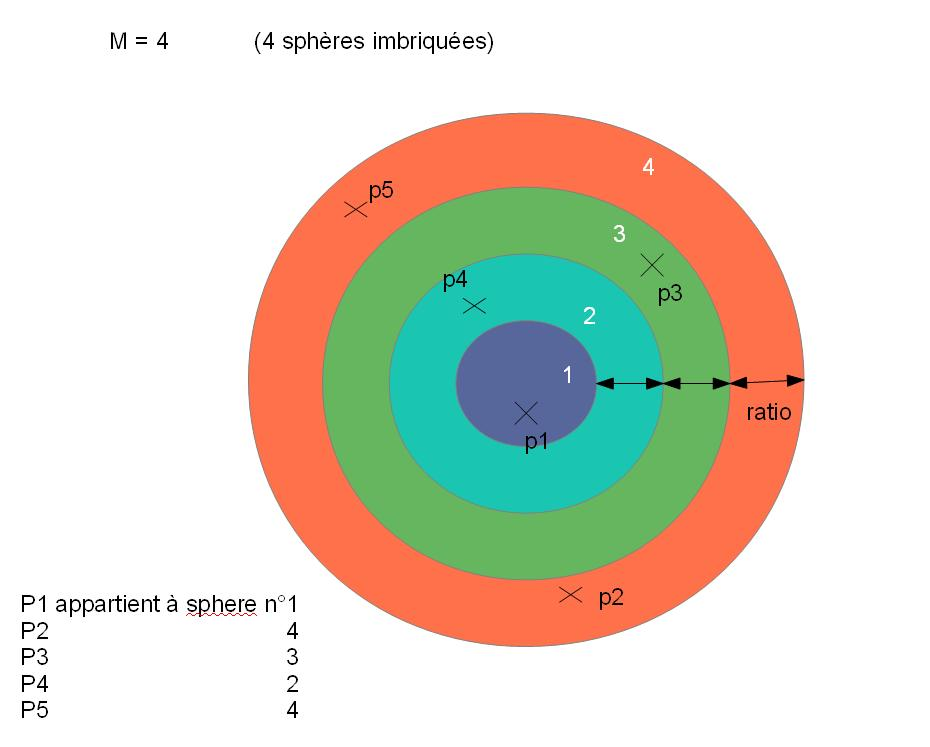
\includegraphics[width=0.8\columnwidth]{Cercle_imbrique.jpg}
    \caption{GPS space division (image taken from \href{https://ensiwiki.ensimag.fr/index.php?title=Descripteur_de_formes_et_mouvements_3D_et_classification_d\%27animations}{here})}
    \label{fig:m_spheres}
\end{figure}

Then we compute the \emph{G2} distributions defined as the histogram of pairwise distances between the points uniformly sampled in 2 regions. By this operation, we can construct $m(m+1)/2$ histograms for each region combination. By computing then the distances between histograms of different shapes we can compute how distinct they are as their spectrum substantially changes beyond the threshold of a mesh deformation (such as pose changes, small topology changes, etc.)


\section{Implementation}

\subsection{General pipeline}

In order to implement the two methods described in the previous sections, we proceeded in two stages:
\begin{itemize}
    \item Firstly, we use the \emph{libigl} library \cite{Libigl} in C++, presented throughout the course, to read, load in memory, compute the Laplacian and its eigen-decomposition via the methods \texttt{igl::cotmatrix}, \texttt{igl::massmatrix} and \texttt{igl::eigs}. Once we have the corresponding spectra, we build the GPS matrices and shapeDNA vectors for each mesh file and save them to a text file.
    \item Secondly, we read the computed spectra using Python and process them to compute the $m$ regions, the corresponding histograms, distances and dimensionality reduction to visualize the different embeddings' performance.
\end{itemize}

We decided to work under this scheme because of the mesh-processing capabilities of \emph{libigl}, mainly the memory-efficient laplacian computation and matrix eigen-decomposition via sparse matrix data structures (although this last was not that robust), and also because of Python's almost ready-to-go array manipulation and data visualization functions to compute the histograms and plots.

Additionally, we used a driver file written in python to distribute the calculation of GPS and Shape-DNA descriptors on the computers from the lab rooms. Since there are about 200 computers in these rooms, all with good CPUs, the calculation was extremely efficient and we are quite sure that this pipeline could scale extremely well to bigger datasets, and we were able to do our calculations on the Princeton segmentation dataset. A further optimisation step could be to try to make use of the GPUs that are on these computers too.

\begin{figure}[H]
    \centering
    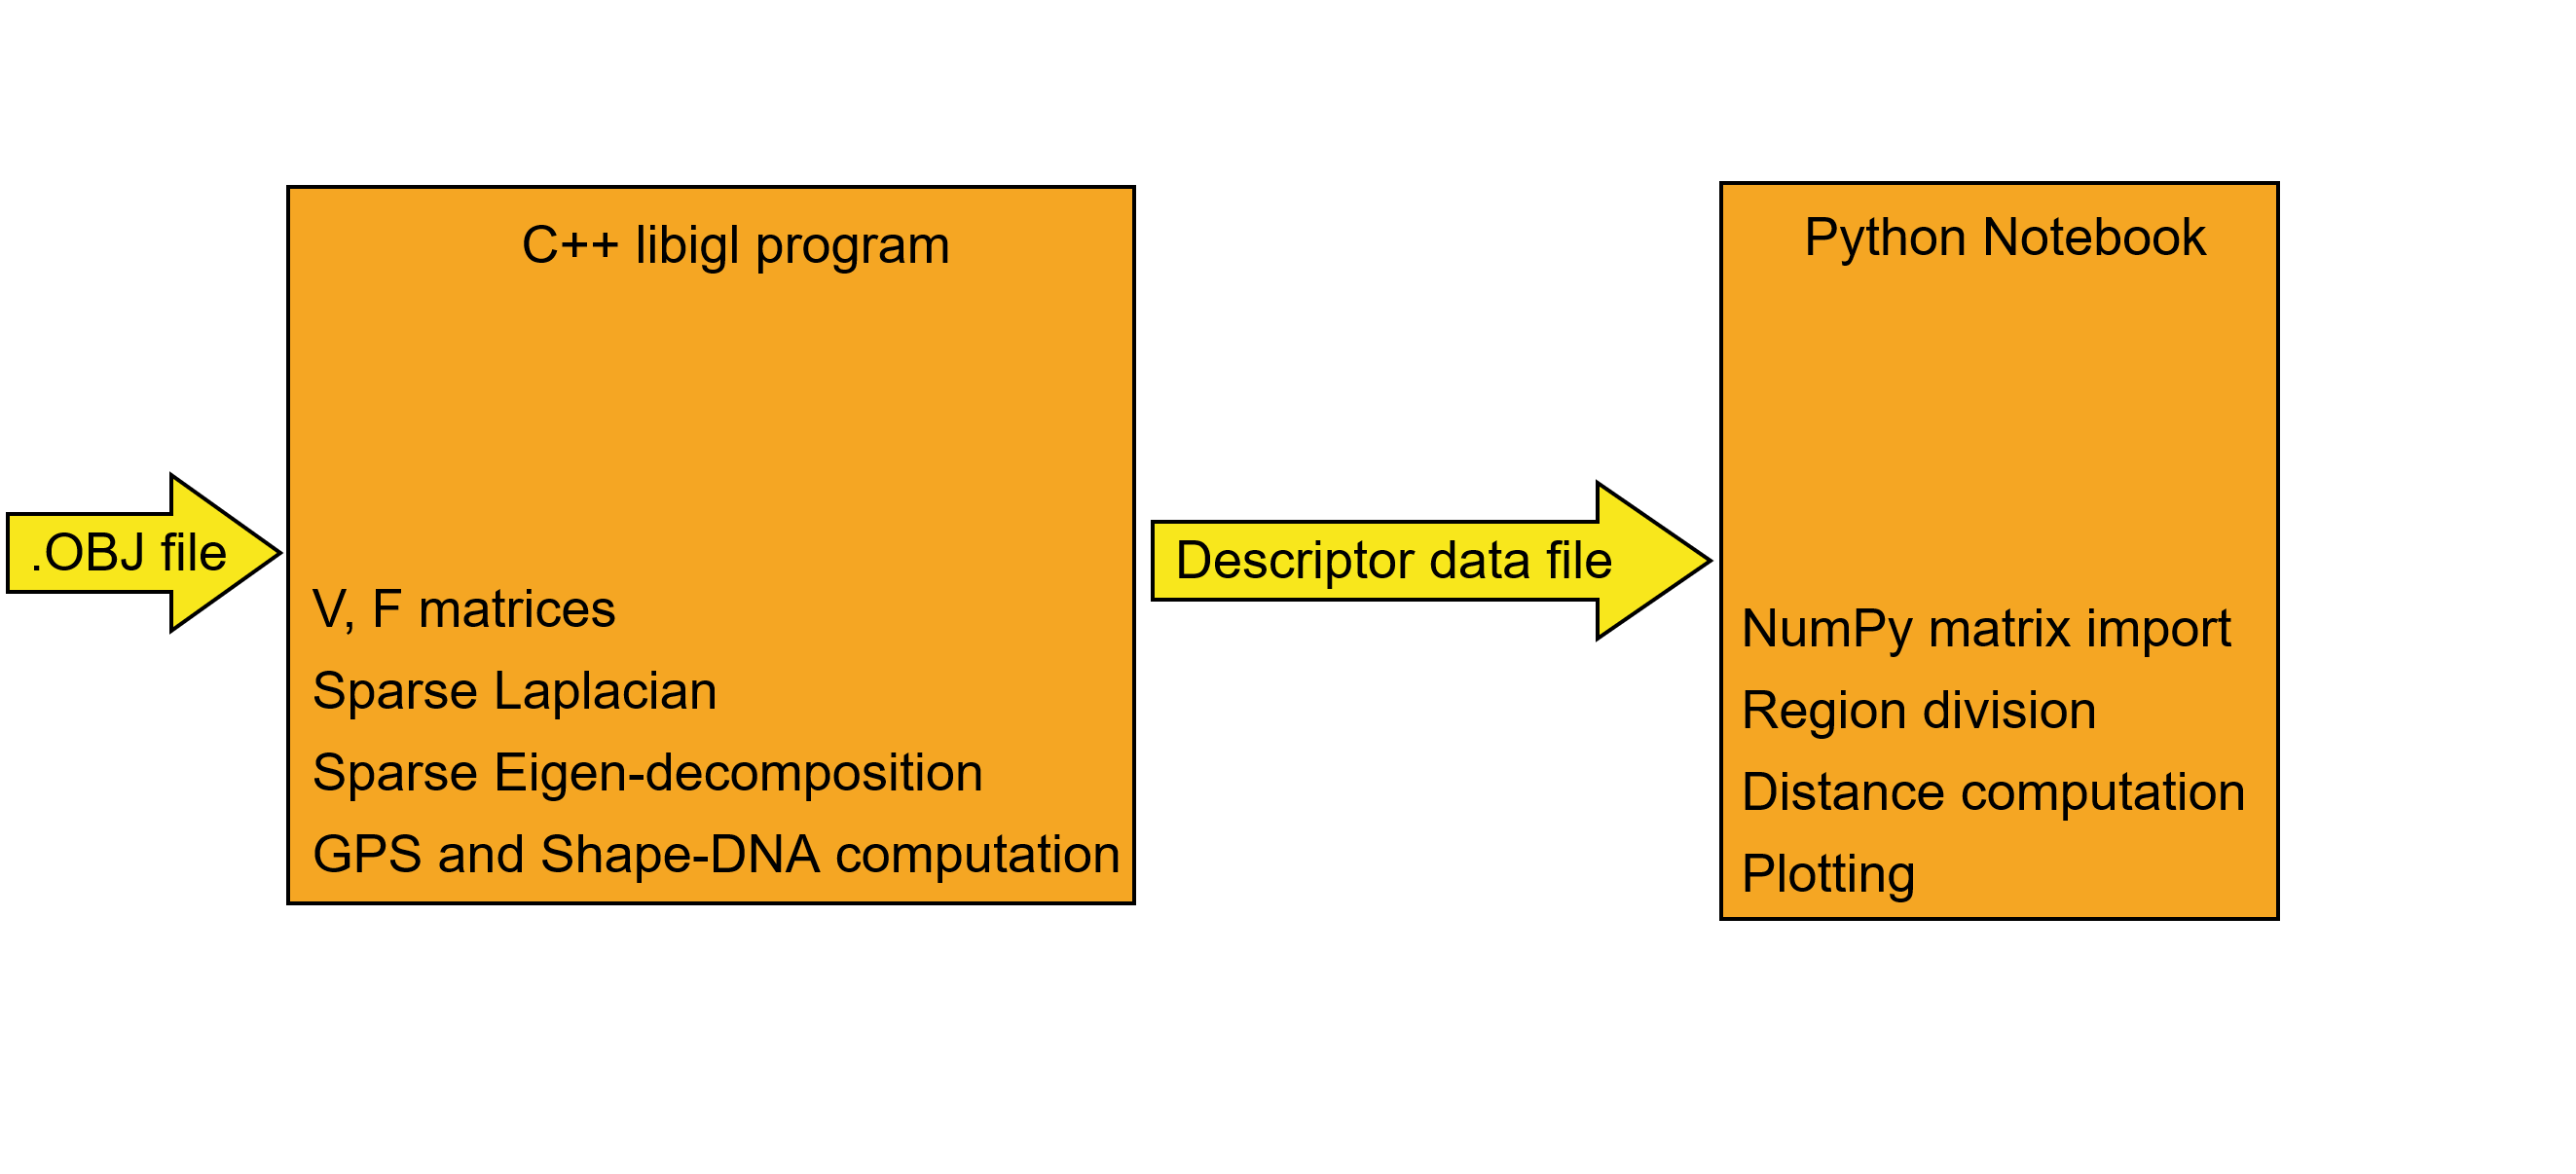
\includegraphics[width=\columnwidth]{pipeline_diagram.png}
    \caption{Implemented 2-stages pipeline}
    \label{fig:pipeline}
\end{figure}

\subsection{Descriptor computation}

By this framework, the executable program compiled from \texttt{main.cpp} receives 2 arguments, an \texttt{.OBJ} file path and a desired depth of the spectrum to compute. We specify that this is a desired depth because the \texttt{igl::eigs} method may fail to converge in the eigen-decomposition computation. This is because the \emph{libigl} implementation is a simplified version of MATLAB's \href{https://www.mathworks.com/help/matlab/ref/eigs.html}{eigs} function so we only have an iterative Power Method in \emph{libigl}.

%TODO: Use a bibliography ref for the link, because it is not really visible
%done in href package calling at preamble
If \texttt{igl::eigs} doesn't converge for a given mesh and $d$, we smooth the laplacian matrix and prune the \q{too small} values using the size-normalized Frobenius norm to decide (inspired by \href{https://www.mathworks.com/matlabcentral/answers/172633-eig-doesn-t-converge-can-you-explain-why}{this} topic in MATLAB forums) and if the eigen-decomposition of this smoothed matrix fails to converge again, we reduce by 1 the depth and we start the computation again.

Finally, we launched this script both in our own computers to test it and in the \emph{Salles Info} via SSH and then we recovered the files to proceed with their analysis.

\subsection{Descriptor analysis}

The second script works through a Jupyter Notebook where we defined the necessary functions to import the descriptors produced in the previous program as an \href{https://docs.scipy.org/doc/numpy/reference/arrays.ndarray.html}{\texttt{ndarray}}, divide the descriptors in regions (as described in \ref{GPS_section}), sample the GPS embeddings, estimate the density from a given distance distribution via a Gaussian Kernel Density Estimation, a wrapper for three dimensionality reduction methods (Multidimensional Scaling -- MDS, Principal Component Analysis -- PCA and t-Distributed Stochastic Neighbor Embedding -- t-SNE) and plotting functions to show annotated scatter plots (for Shape-DNA vectors) and histograms (for GPS embeddings).

For this to work, we specify in the script the $m$ regions to divide the GPS space, the proportion of points to be sampled, the relative paths to descriptor files and the seed to be used in all random-based computations.

\section{Results}

We applied the implementation described above in the \q{Mesh Data from Deformation Transfer for Triangle Meshes} dataset \cite{dataset}, which consists of 337 meshes grouped in 8 objects: \textsf{camel, cat, elephant, face, flamingo, head, horse} and \textsf{lion}.

\begin{figure}[H]
    \centering
    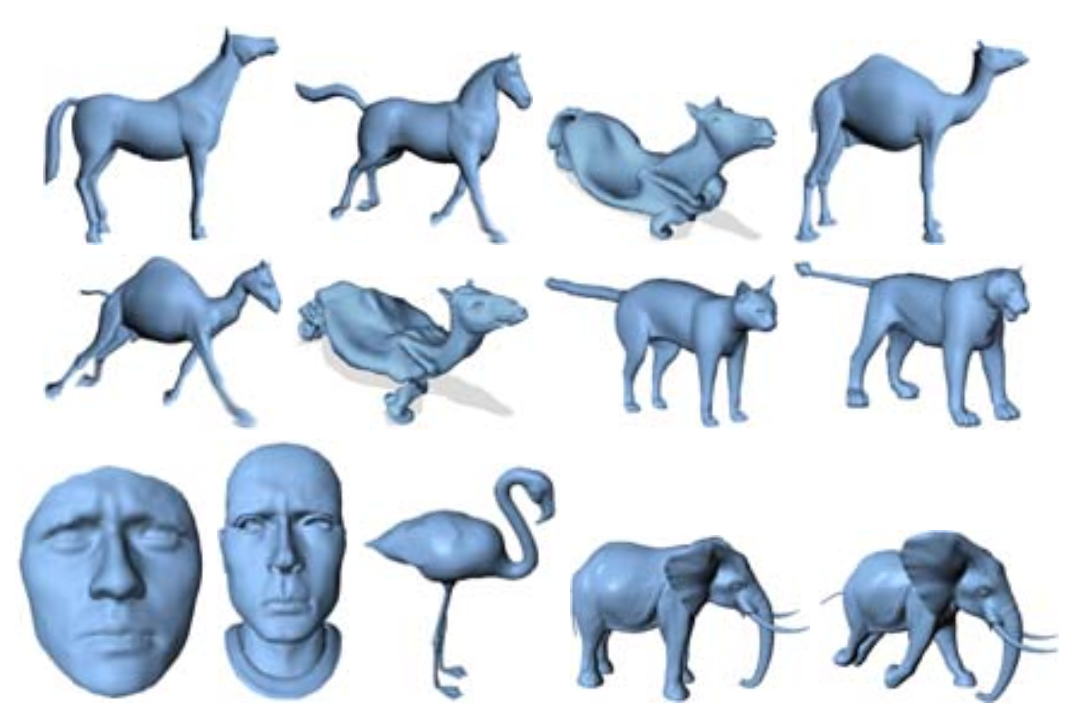
\includegraphics[width=0.7\columnwidth]{dataset_snapshot.png}
    \caption{Snapshot of some of the meshes in the dataset}
    \label{fig:dataset_snap}
\end{figure}

\subsection{Descriptor computation results}

Via the \emph{libigl} available functions, we managed to compute 185 emebeddings ranging from 12 to 20 in the spectrum's depth. This first result is due mainly to the partial eigen-decomposition and the limits imposed by the \texttt{eigs} method (iterations, tolerance). We chose a desired depth of 20 to make some kind of trade-off between the values used for Shape-DNA (50 eigenvalues) \cite{Reuter06} and the ones for GPS (15 eigenvalues) \cite{Rustamov07}.

If we augmented the desired depth beyond 20, we realised that the eigen-decomposition method almost never converged. This is related to the size of the different Laplacian matrices ($\approx 25000 \times 25000$ due to meshes' vertex size) and the iteration limit to approximate the truncated eigen-decomposition (bigger the matrix, slower it is to converge). Although if we increased the maximum iterations, the process became very slow.

We didn't want to explore new eigen-decomposition methods on sparse matrices neither because we thought it escaped the scope of this project. Nevertheless, in order to compare the different embeddings, we had to keep a common spectrum length (of 12) to compare the descriptors.

\subsection{Shape-DNA}

We found that with a relatively small descriptor size (12 compared to 50 in the original publication), it was possible to obtain \q{clusters} of shape descriptors that correspond to the same base shape (among the 8 types listed earlier). With a PCA dimesionality reduction we obtained the most neat groups:

\begin{figure}[H]
    \centering
    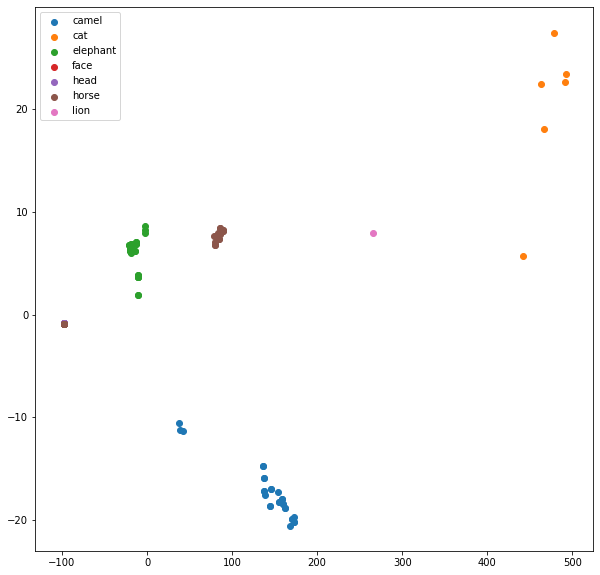
\includegraphics[width=0.9\columnwidth]{pca_simple.png}
    \caption{PCA on Shape-DNA vectors (size 12), only base shape tags}
    \label{fig:pca_simple}
\end{figure}

With MDS (the visualization proposed in \cite{Reuter06}) we have a similar representation but the \textsf{camel} region is no longer convex (\textsf{horse} is in-between):

\begin{figure}[H]
    \centering
    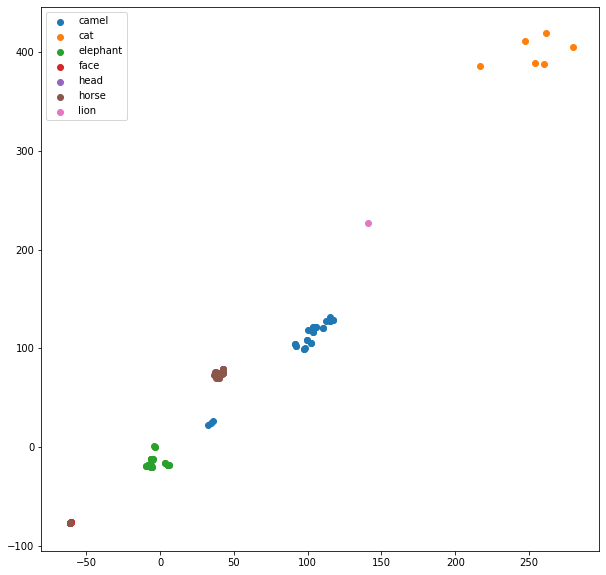
\includegraphics[width=0.9\columnwidth]{mds_simple.png}
    \caption{MDS on Shape-DNA vectors (size 12), only base shape tags}
    \label{fig:mds_simple}
\end{figure}

In both cases, it's difficult to distinguish between one of \textsf{horse} and \textsf{face}. This can be due to the length of the descriptor (i.e. very close in low-frequency eigenvalues).

\subsection{Global Point Signature}

We saw in the previous subsection that the Shape-DNA embeddings could be very sensitive to the pose of an object (namely in \textsf{camel}), which is one of the properties that GPS embeddings tries to revert via the eigen-vector normalization and the random sampling in the $m$ regions. For visualization purposes, we used $m=1$.

In the case of the \textsf{head} meshes:

\begin{figure}[H]
    \centering
    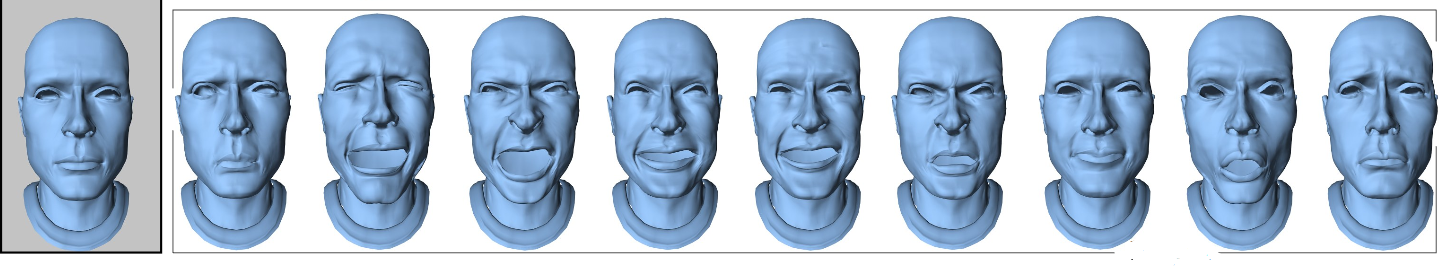
\includegraphics[width=\columnwidth]{head_all.png}
    \caption{All \textsf{head} poses, image taken from \cite{Sumner04}}
    \label{fig:head_all}
\end{figure}

We obtained an astonishingly accurate result in the proximity between the distance histograms:

\begin{figure}[H]
    \centering
    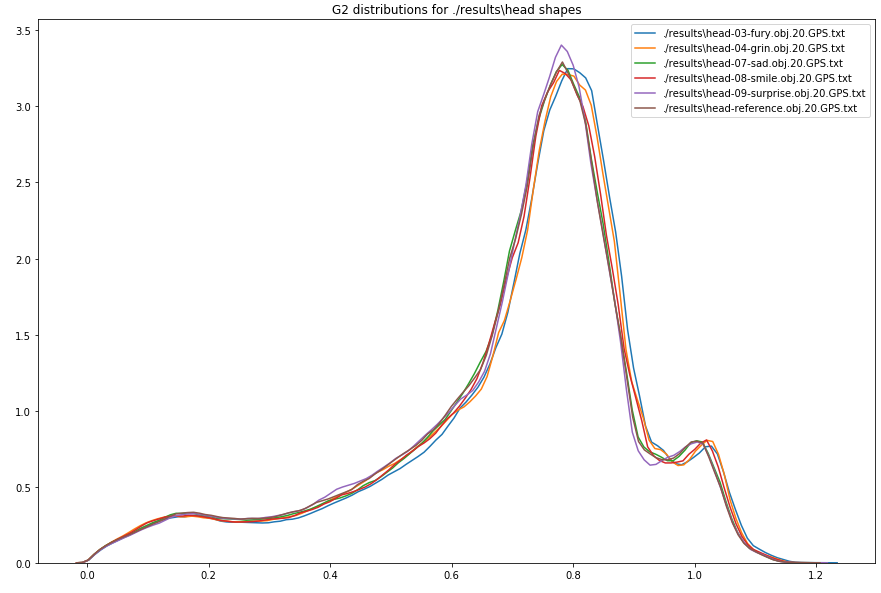
\includegraphics[width=0.9\columnwidth]{face_gps.png}
    \caption{Gaussian-KDE for GPS distances histogram ($m=1$), all \textsf{head} poses}
    \label{fig:face_gps}
\end{figure}

This effect is seen across all types of objects but with different degrees of proximity. For instance, for the \textsf{cat} meshes:

\begin{figure}[H]
    \centering
    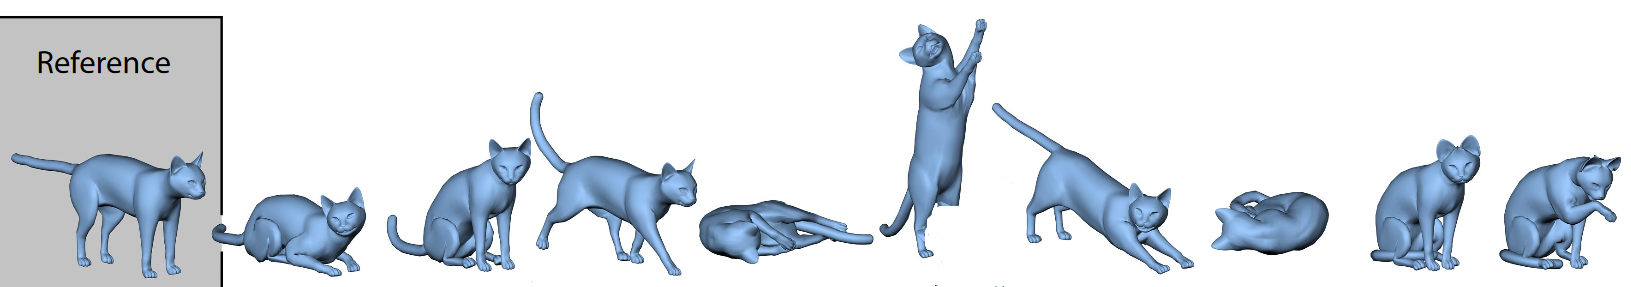
\includegraphics[width=\columnwidth]{cat_all.png}
    \caption{All \textsf{cat} poses, image taken from \cite{Sumner04}}
    \label{fig:cat_all}
\end{figure}

We obtain more different distance histograms:

\begin{figure}[H]
    \centering
    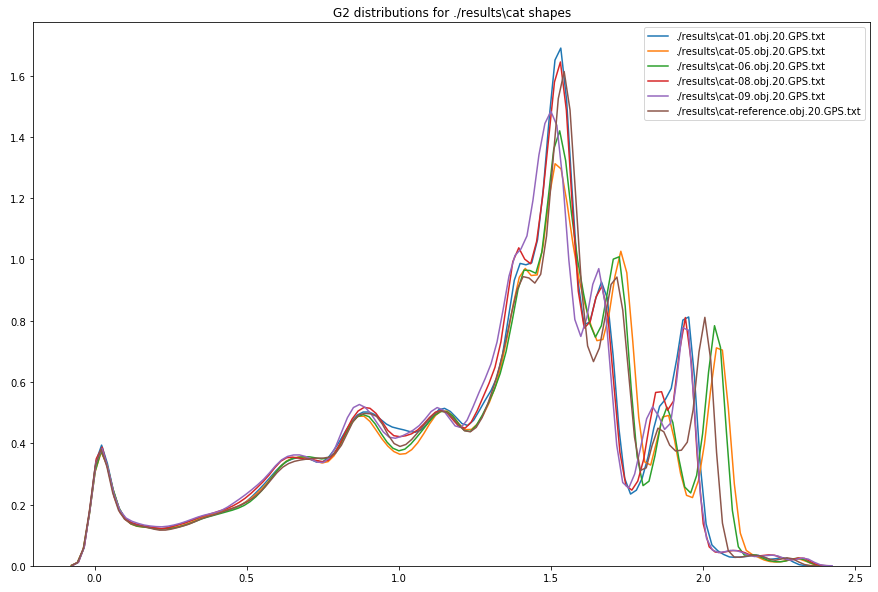
\includegraphics[width=0.9\columnwidth]{cat_gps.png}
    \caption{Gaussian-KDE for GPS distances histogram ($m=1$), all \textsf{cat} poses}
    \label{fig:cat_gps}
\end{figure}

This can be partly explained by the different poses for \textsf{head} and \textsf{cat}. In the latter, the mesh has long extremities (legs) that offer a different type of deformations. Nevertheless, solely the distance histogram offers a sort of \q{profile} for each type of shape, which can be compared with others (just as the frequency signature of a song, for example).

We then computed a dissimilarity mesure between meshes using the kolmogorov smirnov test for empirical distributions, allowing us to compute a MDS of datasets.


\section{Conclusion}

Both descriptors Shape-DNA and GPS proved to be accurate with respect to isometry, similarity and compression along the studied meshes. Although the original implementations described in \cite{Rustamov07} and \cite{Reuter06} didn't mention how to implement all the comparisons and distributions, we show a simplified pipeline and provide the code to do it.


% Can use something like this to put references on a page
% by themselves when using endfloat and the captionsoff option.
\ifCLASSOPTIONcaptionsoff
  \newpage
\fi



% trigger a \newpage just before the given reference
% number - used to balance the columns on the last page
% adjust value as needed - may need to be readjusted if
% the document is modified later
%\IEEEtriggeratref{8}
% The "triggered" command can be changed if desired:
%\IEEEtriggercmd{\enlargethispage{-5in}}

% references section

% can use a bibliography generated by BibTeX as a .bbl file
% BibTeX documentation can be easily obtained at:
% http://www.ctan.org/tex-archive/biblio/bibtex/contrib/doc/
% The IEEEtran BibTeX style support page is at:
% http://www.michaelshell.org/tex/ieeetran/bibtex/
%\bibliographystyle{IEEEtran}
% argument is your BibTeX string definitions and bibliography database(s)
%\bibliography{IEEEabrv,../bib/paper}
%
% <OR> manually copy in the resultant .bbl file
% set second argument of \begin to the number of references
% (used to reserve space for the reference number labels box)

\bibliography{biblio} 
\bibliographystyle{IEEEtran}

\end{document}


